% This is samplepaper.tex, a sample chapter demonstrating the
% LLNCS macro package for Springer Computer Science proceedings;
% Version 2.25 of 2026/09/03
%
\documentclass[runningheads]{llncs}
%
\usepackage[T1]{fontenc}
% T1 fonts will be used to generate the final print and online PDFs,
% so please use T1 fonts in your manuscript whenever possible.
% Other font encondings may result in incorrect characters.
%

\usepackage{newtxtext}       %
\usepackage{amsmath}
\usepackage[varvw]{newtxmath}       % selects Times Roman as basic font

%\hypersetup{hidelinks}
\usepackage[hidelinks]{hyperref}
\usepackage{graphicx}
\usepackage{placeins}
\usepackage{array}
\usepackage{xurl}
\setlength{\emergencystretch}{2em}
% Used for displaying a sample figure. If possible, figure files should
% be included in EPS format.
%
% If you use the hyperref package, please uncomment the following two lines
% to display URLs in blue roman font according to Springer's eBook style:
%\usepackage{color}
%\renewcommand\UrlFont{\color{blue}\rmfamily}
%\urlstyle{rm}
%
\begin{document}
%
\title{Producer Activity, Content Adaptation, and Relative Exposure}
%
\titlerunning{Content Adaptation and Relative Exposure}
% If the paper title is too long for the running head, you can set
% an abbreviated paper title here
%
\author{Kajetan Karbowski (s5470161) \and
Karolina Kozikowska (s5504503)}
%
% First names are abbreviated in the running head.
% If there are more than two authors, 'et al.' is used.
%
\institute{Design of Multi-Agent Systems, University of Groningen}
%
\maketitle              % typeset the header of the contribution
%
\begin{abstract}
High-volume AI-generated content motivates a distinction between producing more content and selecting content using feedback. We extend DOCES with weighted activity, post provenance and an \(\varepsilon\)-greedy opinion-selection policy based on past receipts per accepted original post. The existing 10,000-world activity sweep shows a small moderate-activity exposure excess and attenuation at high activity with a one-item feed. A new experiment compares baseline, random-bin and adaptive producers across 200 paired worlds and 7,200 runs. In the one-item-feed grid, all mean adaptive-minus-control changes in relative exposure \(D=S_{\mathrm{exposure}}-S_{\mathrm{production}}\) are negative; six of 16 comparisons remain significant after Holm correction across 24 policy contrasts. At 10\% prevalence and \(10\times\) activity, adaptation raises both production and receipt shares, but lowers \(D\) by 0.0109 relative to baseline. Descriptive diagnostics show higher posting acceptance and receipts per attempt without higher receipts per accepted post. We do not resolve an interaction between policy and activity, or a policy effect with larger feeds. These findings concern one scalar-opinion feedback mechanism, not actual media quality, engagement or the full AI-slop production cycle.
\keywords{Multi-agent systems \and Synthetic content \and Information diffusion \and Social media \and Agent-based modelling \and AI slop}
\end{abstract}

\section{Introduction}

Generative AI enables online content producers to produce content at a scale that would previously have required substantially more manual effort~\cite{tang2026}. This has contributed to the growth of high-volume AI-generated material that is often described as AI slop. We use the term \emph{AI slop} for the motivating real-world phenomenon, while the model represents content more generally as human- or synthetic-origin content. Recent ethnographic work by Tang et al.~\cite{tang2026} shows that some producers systematically benchmark viral content, test variations, operate multiple accounts, and prioritise speed, scale, and adaptability over stable authorship or identity.

A high production volume alone does not tell us how much synthetic content users actually receive. Social-media content spreads through interactions between producers, users, social connections, reposting behaviour, and recommendation systems. A minority of highly active producers may therefore obtain either more or less exposure than their raw production share would suggest.

The distinction matters because a large share of synthetic content in users' feeds can arise for different reasons. Synthetic producers may simply create more posts, or network and platform dynamics may give those posts more exposure than their production share would predict. These mechanisms have different implications for understanding high-volume AI-generated content. Empirical work on AI-slop production documents strategies centred on scale, rapid iteration, and attention capture~\cite{tang2026}, while Pendergrass et al.~\cite{pendergrass2025} frame user attention as a scarce resource for which such content competes. We therefore study not only how much synthetic content is produced, but how efficiently that production translates into exposure.

We study the following research question:

\begin{quote}
\textit{How do synthetic-producer activity and receipt-based content adaptation affect relative exposure in an adaptive social-network simulation?}
\end{quote}

We define relative exposure as
\[
D = S_{\mathrm{exposure}} - S_{\mathrm{production}},
\]
where positive values indicate that synthetic-origin content receives a larger
share of feed exposure than its share of production, while negative values
indicate attenuation.

We address the main question through three subquestions:
\begin{enumerate}
\item \textit{SQ1: Activity.} How does activity affect production and receipt shares when synthetic producers do not adapt their content?
\item \textit{SQ2: Adaptation.} Does receipt-based content selection change relative exposure compared with baseline and random-strategy producers at the same activity level?
\item \textit{SQ3: Interaction.} Does adaptation change the contrast between moderate and high activity, and does its effect depend on feed capacity?
\end{enumerate}

In the present experiment, ``synthetic'' denotes the provenance of posts introduced by a randomly assigned producer subgroup. In the activity-only baseline, these agents follow the same content-generation rules as other agents. The new adaptive condition additionally changes their choice of content opinion in response to prior receipts. Posting and receiving filters, opinion updating, reposting, and rewiring remain common across producer policies. The label could equally identify another high-activity producer group; the simulator does not generate or classify AI content.

Our contribution combines the existing activity study with a controlled test of feedback-responsive opinion selection. We compare adaptive producers with both the original baseline and a random-bin control. We also test feed-capacity sensitivity. We do not generate or evaluate actual images, videos, or text, and we do not test whether AI generation itself causes amplification.

These questions are measurable through production, feed-receipt, and activity statistics recorded by the simulation. We first vary producer prevalence and activity, then compare content policies at matched activity while measuring production, receipt and attempt-based outcomes.

A multi-agent model is appropriate because relative exposure is not determined by producer activity alone. It emerges from repeated interactions between heterogeneous users, posting and reposting, limited feeds, content filtering, opinion dynamics, and adaptive network connections. The simulation allows us to vary producer activity while holding the remaining model mechanisms fixed.

\section{Related Work}

\subsection{Information diffusion and opinion dynamics}
Our main computational starting point is the model by Oliveira et al.~\cite{oliveira2026}. Their agent-based model combines information diffusion with opinion dynamics on an adaptive social network. Agents have limited feeds, create or repost content, receive content according to filtering rules, update their opinions, and may rewire social connections. The authors show that reposting, recommendation rules, and the probability of introducing new content can substantially change both cascade dynamics and final opinion distributions.

This model is particularly useful for our research because it explicitly links individual posting behaviour to network-level information diffusion. It also provides an existing mechanism for recommendation, reposting, limited attention, and adaptive network structure.

We use the DOCES implementation developed by de Arruda et al.~\cite{deArruda2025}. DOCES provides the adaptive social-network simulation and supports recommendation rules, changes in friendships, and opinion dynamics.

\subsection{Critical review of Oliveira et al.}
Oliveira et al. provide a strong starting point because their model separates several mechanisms that are often combined in empirical social-media data. The authors can independently manipulate content innovation, recommendation, rewiring, and opinion updating. They also compare simulated cascade distributions with empirical data, which gives the model more grounding than a purely abstract diffusion model.

The model nevertheless makes one simplifying assumption that is central to our research question: users are selected uniformly for activation. All users therefore have the same opportunity to create or repost content. Oliveira et al.~\cite{oliveira2026} explicitly identify heterogeneous activity and bursty dynamics as directions for future work.

This assumption is poorly suited to the production practices described by Tang et al.~\cite{tang2026}, where some AI-supported producers operate at high volume. We therefore retain the Oliveira diffusion dynamics but replace uniform activation with heterogeneous activity weights.

\subsection{Synthetic content and the attention economy}

Tang et al.~\cite{tang2026} provide behavioural grounding for our synthetic producers. Their ethnographic study of AI-slop creators in China describes production practices based on high output, repeated experimentation, benchmarking successful formats, matrix account systems, and algorithmic opportunism. Their findings suggest that AI-supported production can make speed and scale central features of online content production.

Pendergrass et al.~\cite{pendergrass2025} describe a related conceptual feedback process. They argue that cheap AI production, attention-oriented content, platform distribution, and economic incentives can form a self-reinforcing cycle. Their framework emphasizes that generated content competes for attention and that successful attention strategies create incentives for further production.

These studies serve different roles. Tang et al. provide qualitative motivation for heterogeneous activity; they do not supply numerical values for our activity multipliers. Pendergrass et al. provide a conceptual account of creation, distribution, and reward, rather than an empirically calibrated diffusion rule. We model a fixed activity advantage and one limited feedback mechanism: producers select opinion ranges using previous feed receipts. This does not reproduce the full production--distribution--financial-reward cycle. Producer adaptation is an additional mechanism, distinct from DOCES follower rewiring.

\subsection{Research gap}

The three strands of work provide complementary pieces of the problem. Oliveira et al.~\cite{oliveira2026} provide a mechanistic model of posting, reposting, recommendation, limited attention, opinion change, and adaptive network structure, but assume uniform user activation. Tang et al.~\cite{tang2026} document synthetic-content production practices centred on high output and rapid experimentation, while Pendergrass et al.~\cite{pendergrass2025} emphasise competition for limited attention.

What remains unclear is how a systematically high-activity producer population affects exposure once its content enters an adaptive social network. In particular, higher production need not imply proportionally higher exposure. We extend the Oliveira--DOCES framework first with heterogeneous activity and provenance, then with receipt-responsive content selection. The controlled policy comparison tests whether a specific feedback mechanism changes exposure beyond the effect of high activity.

\section{Method}

\subsection{Base model}

We build on the adaptive social-network model of Oliveira et al.~\cite{oliveira2026}, using its DOCES implementation by de Arruda et al.~\cite{deArruda2025}. Each user \(i\) is a node in a directed network and holds a continuous opinion \(b_i\in[-1,1]\). Each piece of content has a fixed opinion value \(\theta\in[-1,1]\), and each user maintains an ordered feed (memory) of size \(\alpha\).

The following rules define the baseline. The adaptive extension changes only how synthetic innovation attempts select \(\theta\), as specified in Section~\ref{sec:producer-policy}. One simulation iteration consists of five stages. First, one user \(i\) becomes active. In the original model this user is selected uniformly; our heterogeneous-activity extension modifies only this stage. Second, with probability \(\mu\), the active user creates new content whose opinion \(\theta\) is sampled uniformly from \([-1,1]\). With probability \(1-\mu\), the active user instead selects the highest-priority item in its feed for reposting, provided the feed is non-empty. The selected item's feed priority is subsequently rotated to the lowest priority. In the main sweep, \(\alpha=1\), so this reordering has no effect on which item remains in the feed. It matters in the larger-feed sensitivity conditions.

Posting is accepted probabilistically according to the conflicting-posting filter used by Oliveira et al.:
\[
P_p(\theta,b_i)=
\cos^2\left(\frac{\pi}{2}|\theta-b_i|\right).
\]
If the post is made, each follower \(j\) independently receives it according to
\[
P_r(b_i,b_j,\phi)=
\cos^2\left(\frac{\pi}{2}|b_i-b_j|+\phi\right),
\]
where \(\phi\) controls the receiving rule and acts as a stylised proxy for platform recommendation. The filter acts only on existing follower links. It does not rank candidate content or recommend posts outside this network. At \(\phi=\pi/2\), it favours opinion distances near 1 and suppresses distances near 0 and 2; it is not a general measure of recommendation strength. A post that passes the filter enters the top of a follower's feed only if it is absent there. When the feed is full, insertion removes the lowest-priority item. DOCES can still update a recipient's opinion after filter acceptance when the post is already present; such an interaction adds no receipt to our exposure measure.

Recipients update their opinions through either attraction to or repulsion from the received post. With the opinion range fixed to \([-1,1]\), the probability of attraction for recipient \(j\) is
\[
P_{\mathrm{attr}}(\theta,b_j)
    = 1-\frac{|\theta-b_j|}{2},
\]
and repulsion occurs otherwise. Under attraction, \(b_j\) moves by at most \(\Delta\) towards \(\theta\), without overshooting the post opinion. Under repulsion, \(b_j\) moves by \(\Delta\) away from \(\theta\) and is clipped to the interval \([-1,1]\). No stubborn agents are used in the reported experiments.

When rewiring is enabled, DOCES considers rewiring only after a repulsive interaction. Let \(b'_j\) denote the recipient's opinion after repulsion and let \(y=|b_i-b'_j|\) be its distance from the active user's opinion. Rewiring is possible only when \(y>1\). In the implementation used here it occurs when
\[
u > \cos^2\left(\frac{\pi}{2}y\right),
\qquad u\sim U(0,1).
\]
Equivalently, conditional on \(y>1\), the implemented rewiring probability is \(1-\cos^2(\pi y/2)\). When rewiring succeeds, the existing follower connection to the active user is replaced by a connection to a randomly sampled eligible user; the current source, the recipient itself, and already-connected targets are excluded. Thus information diffusion, opinion dynamics, and network structure can co-evolve during a simulation.

\subsection{Baseline parameterisation}

Unless otherwise stated, all reported experiments use
\[
N=1000,\qquad
\mu=0.1,\qquad
\phi=\frac{\pi}{2},\qquad
\Delta=0.1,\qquad
\alpha=1,
\]
with rewiring enabled and 100,000 requested iterations per simulation. The inherited inclusive loop executes 100,001 activations for this request. We retain this convention in both experiments. Initial
opinions are sampled independently and uniformly from \([-1,1]\). Agents are
connected by a directed Erdős--Rényi graph. For each ordered pair of distinct
agents, an edge is sampled independently with probability
\[
p=\frac{10.21}{N-1},
\]
giving a target mean in-degree of 10.21.

These choices are inherited from the Oliveira et al. parameterisation used in our baseline validation rather than fitted to synthetic-content data. In particular, Oliveira et al. use an Erdős--Rényi network with \(N=1000\), \(\phi=\pi/2\), \(\Delta=0.1\), and feed size \(\alpha=1\) when characterising the effect of innovation and reposting~\cite{oliveira2026}. We retained this configuration so that heterogeneous activity could be introduced while keeping the remaining diffusion dynamics close to a previously characterised setting.

The Erdős--Rényi network and one-item feed should therefore be interpreted as controlled modelling assumptions, not as literal representations of a specific social-media platform. In particular, \(\alpha=1\) creates a strong limited-attention regime. Section~\ref{sec:feed-design} tests larger feeds. Alternative network structures remain untested.

\subsection{Assumptions and their relevance to AI slop}

We retain the base model to isolate activity, but inherited choices also constrain interpretation (Table~\ref{tab:assumptions}). None of these parameters is fitted to AI-slop traffic.

\begin{table}[tb]
\caption{Model choices, their purpose, and their interpretive limits.}
\label{tab:assumptions}
\centering\small
\begin{tabular}{>{\raggedright\arraybackslash}p{0.22\linewidth}>{\raggedright\arraybackslash}p{0.32\linewidth}>{\raggedright\arraybackslash}p{0.36\linewidth}}
\hline
Choice & Purpose & Limit for AI-slop interpretation \\\hline
Fixed activity weights and random producer labels & Isolate activity and prevalence while comparing content policies & No burstiness, coordinated accounts, or preferential producer placement \\[4pt]
Common innovation probability; baseline uniform opinions & Isolate feedback in opinion selection & No actual media quality, format, or generation cost \\[4pt]
Directed random graph & Allow follower diffusion with controlled initial degree & No calibrated hubs, communities, or real platform network \\[4pt]
Opinion filters and rewiring & Retain feedback between diffusion and user connections & No learned recommender or engagement reward; producer response uses only model receipts \\[4pt]
Finite ordered feeds & Limit retained repost opportunities & Memory is not measured viewing time; capacity also affects repeat-receipt suppression \\\hline
\end{tabular}
\end{table}

Increasing an activation weight increases opportunities to repost as well as to create new posts. It therefore approximates high account activity rather than a pure increase in original-content production. Moreover, the total activation budget is fixed. Increasing synthetic activity lowers the expected number of human activations within that budget. We study a change in relative activity allocation, not additional posts over a calibrated amount of real time.

\subsection{Baseline validation}

Before introducing heterogeneous activity, we validated the simulator against the qualitative behaviour reported in Fig.~2 of Oliveira et al.~\cite{oliveira2026}. Using the corresponding baseline configuration, we ran 50 simulation seeds while holding the network and initial opinions fixed. The low-innovation condition \(\mu=0.1\) produced larger cascades and more frequent bimodal opinion distributions: 15 of 50 runs exceeded the bimodality criterion, compared with 1 of 50 at \(\mu=1\). The median maximum cascade sizes were 2232.5 and 1, respectively. This reproduces a qualitative contrast, not universal polarisation at low innovation. We repeated this baseline after implementing our simulator extensions and obtained the same representative results when activity weighting was disabled. We therefore used this as a regression validation rather than claiming an exact numerical replication.

\subsection{Heterogeneous activity}
We extended DOCES with a relative activity weight \(w_i\) for each user \(i\). The probability of selecting agent \(i\) is

\[
P(i)=\frac{w_i}{\sum_j w_j}.
\]

Human agents receive weight 1. Synthetic agents receive an activity multiplier \(m\). In the original activity sweep, no other behavioural rule depends on the synthetic label. Synthetic and human agents use the same content-creation probability, posting and receiving filters, opinion dynamics, and rewiring rule. The original sweep therefore isolates differences in activation frequency. The follow-up holds these weights fixed while comparing content policies.

For \(N_s\) synthetic and \(N_h\) human agents, the expected synthetic activation share is therefore

\[
S_{\mathrm{activation}} = \frac{N_s m}{N_h + N_s m}.
\]

We validated the implementation independently. A two-agent test with weights 9 and 1 resulted in observed activation shares of approximately 0.900 and 0.100 over 100,001 selections.

When activity weights are not configured, DOCES follows its original uniform selection procedure. We reran the Oliveira baseline after the extension and obtained the same representative simulation results.

\subsection{Receipt-responsive producer policy}
\label{sec:producer-policy}

We add a policy that selects the opinion characteristics of original content. Human producers retain the baseline uniform rule. The synthetic subgroup uses one of three policies: the original uniform baseline, a random-bin control, or a receipt-responsive policy. Activity weights, innovation probability, posting filters and all subsequent diffusion rules are identical between policies.

We partition \([-1,1]\) into five equal-width opinion bins. After selecting bin \(a\in\{0,\ldots,4\}\), a synthetic producer draws \(\theta\) uniformly from that bin. The random control chooses every bin with probability \(1/5\). Its marginal opinion distribution is therefore uniform, like the original baseline, but its sampling uses an additional random draw. It controls for bin-based sampling without feedback; it is not an additional content-quality treatment.

For producer \(i\) and bin \(a\), let \(P_{ia}(t)\) count accepted original posts created before the current choice, and let \(R_{ia}(t)\) count their receipts observed up to that time. We use
\[
Q_{ia}(t)=\begin{cases}
R_{ia}(t)/P_{ia}(t), & P_{ia}(t)>0,\\
0, & P_{ia}(t)=0.
\end{cases}
\]
We use an \(\varepsilon\)-greedy exploration rule~\cite{sutton2018}. With probability \(\varepsilon=0.1\), the adaptive producer chooses a bin uniformly. Otherwise, it chooses a bin with maximum \(Q_{ia}\), breaking ties uniformly. The policy acts only on innovation attempts, not on repost selection. Its scores update as receipts arrive, including later receipts generated by other users reposting the producer's original content. Background posts provide no reward. A rejected innovation attempt increments the attempt counter but does not create a post or enter the score denominator.

This is a cumulative receipt-per-accepted-post objective. It does not directly optimize posting acceptance or receipts per attempt. The rule has no forgetting, explicit update window or financial reward. Older posts have more time to receive feedback, recent posts are right-censored, and early success can favour continued exploitation. We also assume that a producer can observe all provenance-attributed receipts of its posts, which is stronger than access to many real platform dashboards. The network and other producers also change during the run, so these scores do not estimate fixed, independent strategy rewards. These are deliberate properties of the tested mechanism.

Content adaptation here means selecting scalar opinion ranges. It does not mean learning successful videos, visual formats or semantic topics. Moreover, the receiving filter uses the sender's and recipient's opinions, not \(\theta\) directly. Changing \(\theta\) can affect posting acceptance, later repost acceptance, opinion dynamics and the subsequent network trajectory. We therefore measure these outcomes separately instead of interpreting a receipt increase as direct targeting by a recommender.

Tests verify that the greedy rule changes its choice when reward histories change, that full exploration samples every bin, and that accepted-post and receipt counters reconcile with post-level provenance. Configuring tracking with the baseline policy preserves the original trajectory exactly. We also reran the 50-seed baseline and reproduced its saved aggregate results after the extension.

\subsection{Post provenance and exposure}
Each newly created post stores the identifier of its original creator. Reposts retain both the post identifier and original creator, so exposure is attributed to the producer that originally introduced the content rather than to the user currently reposting it.

DOCES initializes each feed with \(\alpha\) distinct background posts. We assign these posts an origin ID of \(-1\) and exclude them and their receipts from the human-versus-synthetic measurements. They still occupy feeds and can be reposted, so they influence subsequent dynamics. Larger capacities therefore also increase the initial background stock from \(N\) to \(N\alpha\) posts.

We define one model-level exposure event as a successful insertion of a post into another user's feed. The receiving filter must accept the post, and the same post must not already be in the recipient's feed. We do not count insertion into the posting user's own feed as exposure.

This measure represents successful feed receipt inside the model. It should not be interpreted as an exact real-world impression or view.

\subsection{Outcome measures}
We measure synthetic production share as

\[
S_{\mathrm{production}} = \frac{N_{\mathrm{synthetic\ posts}}} {N_{\mathrm{synthetic\ posts}}+N_{\mathrm{human\ posts}}}.
\]

Synthetic exposure share is

\[
S_{\mathrm{exposure}} = \frac{R_{\mathrm{synthetic}}} {R_{\mathrm{synthetic}}+R_{\mathrm{human}}},
\]

where \(R\) is the number of successful feed receipts. Production counts distinct new posts accepted by the posting filter, not rejected creation attempts or reposts. A post can contribute several receipts to the same recipient if it leaves that feed and is later reinserted. Receipts therefore measure neither unique audience reach nor time spent viewing content.

Our primary outcome is

\[
D = S_{\mathrm{exposure}}-S_{\mathrm{production}}.
\]

A positive value indicates that synthetic content obtains more exposure than its production share. A negative value indicates attenuation.

To examine how efficiently additional production translates into exposure, we also calculate mean receipts per post separately for synthetic and human content:
\[
E_s = \frac{R_{\mathrm{synthetic}}}{N_{\mathrm{synthetic\ posts}}},
\qquad
E_h = \frac{R_{\mathrm{human}}}{N_{\mathrm{human\ posts}}}.
\]

We use
\[
G_E = E_s-E_h
\]
as an exposure-efficiency gap. A positive value means that the average synthetic-origin post receives more successful feed receipts than the average human-origin post; a negative value means it receives fewer. These measures are algebraically related. If \(q=S_{\mathrm{production}}\), then, whenever the denominators are positive,
\[
D=\frac{q(1-q)(E_s-E_h)}{qE_s+(1-q)E_h}.
\]
Thus the signs of \(D\) and \(G_E\) agree by construction; they are not independent evidence for a causal mechanism.

For the adaptive comparison, let \(T_s\) denote synthetic innovation attempts. We additionally measure posting acceptance \(A_s=P_s/T_s\) and receipts per attempt \(U_s=R_s/T_s\). Whenever denominators are non-zero, \(U_s=A_sE_s\). These diagnostics distinguish a higher probability of creating an accepted post from a higher receipt count per accepted post; they are related outcomes, not separate causal identifications.

We record strategy selections during the first and last quarters of the run. For each producer observed in both quarters, we calculate the maximum bin share in each quarter. Let \(C\) be the difference between the late and early means of this per-producer maximum share. A positive \(C\) indicates more concentrated later choices. We compare \(C\) across policies because finite samples alone create concentration, especially when individual producers make few attempts.

\subsection{Experimental design}

We test synthetic-producer prevalence values of
\[
1\%,\;5\%,\;10\%,\;15\%,\;20\%,\;25\%
\]
and relative activity multipliers of
\[
1,\;2,\;3,\;5,\;7.5,\;10,\;15.
\]
A 0\% synthetic control is evaluated at baseline activity. The factorial design therefore contains \(6\times7=42\) positive-prevalence conditions plus one control, giving 43 conditions in total. The 0\% control is used as an implementation reference and is excluded from factorial prevalence--activity inference because an activity multiplier is not defined for a population containing no synthetic agents.

The four seeds for each world are generated deterministically from master seed \texttt{20260924}. The complete seed manifest is stored with the experiment outputs.

For each world, the master generator produces four separate seeds: a network seed, initial-opinion seed, producer-assignment seed, and simulation seed. All experimental conditions within that world reuse these four seeds. They therefore share the same initial network, initial opinions, producer ordering, and simulation seed. All four seeds change between worlds, creating paired comparisons within worlds while keeping different worlds independent.

We generated 10,000 independent simulated worlds for the final sweep to obtain stable estimates of the condition means and uncertainty intervals. Smaller 2,000- and 5,000-world checkpoints produced the same qualitative relationship; the larger run mainly reduced Monte Carlo uncertainty.

Synthetic groups are nested within each world. A random producer ordering is generated once per world, and larger synthetic populations extend smaller ones. For example, the 5\% synthetic group contains the same agents as the 1\% group plus additional agents. This reduces unnecessary variation in producer identity between prevalence conditions.

The complete design contains
\[
10{,}000 \times 43 = 430{,}000
\]
unique condition-runs.

\subsection{Focused feed-capacity experiment}
\label{sec:feed-design}

We run a separate sensitivity experiment with 200 independent worlds generated from master seed \texttt{20261022}. We cross feed capacities \(\alpha\in\{1,5,20\}\), producer prevalences \(\{5\%,25\%\}\), and activity multipliers \(\{1,3,15\}\). This gives 18 conditions per world and 3,600 condition-runs. We retain the main sweep's network size, degree, filters, innovation probability, opinion update, rewiring, and requested iteration count. Each world shares its graph, initial opinions, nested producer assignment, and simulation seed across conditions.

We selected 3\(\times\) and 15\(\times\) to contrast moderate and high activity after observing the main sweep. The experiment is therefore an exploratory sensitivity analysis. It is not a second 10,000-world sweep or a new search for a turnover threshold. We report pointwise 95\% Student's \(t\) intervals for condition means and for paired within-world differences \(D_{15}-D_3\), without multiplicity adjustment. The same seed does not keep random draws aligned after conditions diverge; different feed sizes also require different numbers of initialization draws.

Changing capacity modifies retention, repost order, duplicate suppression, and the initial stock of background posts together. This experiment tests the bundled feed-capacity assumption. It does not separate feed displacement from other capacity-dependent effects.

\subsection{Adaptive-policy experiment}
\label{sec:adaptive-design}

We generate 200 new independent worlds from master seed \texttt{20261023}. With a one-item feed, we cross prevalences \(\{5\%,10\%\}\), activities \(\{1,2,5,10\}\), and the three policies, giving 24 conditions per world. The additional capacity test crosses \(\alpha\in\{3,5\}\), 5\% prevalence, activities \(\{2,10\}\), and all three policies, giving 12 further conditions. The complete follow-up therefore contains 36 conditions per world and 7,200 runs. The main model parameters and requested horizon remain unchanged.

Within each world, all policy and activity conditions use the same graph, initial opinions, producer ordering and simulation seed. Policies are compared at the same activity and prevalence. Producer sets are nested across prevalence, as in the original sweep. We run fresh paired controls rather than comparing the adaptive sample directly with the earlier 10,000-world means. Different policies consume different numbers of random draws, so shared seeds do not imply step-by-step aligned trajectories. The new worlds are separate from both earlier experiments.

The five bins and \(\varepsilon=0.1\) are simple modelling choices, not values estimated from AI-slop data. We select activity levels to cover the baseline, moderate activity, the earlier turnover region and higher activity. This is a follow-up motivated by the original sweep, not a preregistered test or a new threshold search.

For each prevalence--activity--capacity combination, we estimate adaptive-minus-baseline and adaptive-minus-random paired changes in \(D\). We apply Holm correction across all 24 such comparisons. To address SQ3, we also estimate the within-world difference between the policy effect at \(10\times\) and its effect at \(2\times\). These eight interaction comparisons form a separate Holm family. We report pointwise 95\% Student's \(t\) intervals; they are not simultaneous intervals. Acceptance, receipt efficiency, zero-receipt frequency and strategy concentration are descriptive diagnostics with pointwise intervals in the accompanying data.

\subsection{Statistical analysis}

For each main-sweep condition, we report the mean and a 95\% Student's \(t\) confidence interval for the mean across 10,000 independent worlds. Since activity conditions within each world share the same network, initial opinions, producer ordering, and simulation seed, activity comparisons use paired within-world differences.

For omnibus inference, we represent the \(D\) values from all prevalence-activity conditions as a repeated-measures vector for each world. We test contrasts of the across-world mean vector using its empirical covariance matrix, producing Wald \(\chi^2\) tests for prevalence, activity, and their interaction.

We additionally evaluate exploratory paired activity contrasts using two-sided paired \(t\)-tests. We consider three contrast families: comparisons of each activity level against \(1\times\), comparisons against \(3\times\), and comparisons between adjacent activity levels. Holm's method is applied separately within each family across all tested prevalence levels. For these contrasts we report the mean paired difference, its 95\% confidence interval, and paired Cohen's \(d_z\). Given the large number of independent worlds, interpretation emphasises estimated effect sizes and uncertainty rather than statistical significance alone.

For a paired difference \(\Delta D\), paired Cohen's effect size is
\[
d_z=\frac{\overline{\Delta D}}{s_{\Delta D}}.
\]

For descriptive analysis of the turnover, we identified the tested activity level with the largest mean \(D\) at each prevalence. When mean \(D\) changes sign between two adjacent tested activity levels after this peak, we estimate the zero crossing by linear interpolation between the two condition means. These interpolated values summarise the simulated turnover and are not treated as independently estimated thresholds.

\subsection{Implementation and reproducibility}

The project repository contains the experiment configuration, deterministic seed manifest, experiment and analysis code, summary outputs, and generated figures. The full run-level dataset is retained separately because of its size and can be regenerated from the configuration and seed manifest.

The final volume sweep is configured in \texttt{configs/volume\_sweep\_big.yaml} and orchestrated by \texttt{scripts/run\_big\_volume\_sweep.fish}, which invokes

\texttt{experiments/alpha\_volume\_sweep.py}. Final statistical analysis and figure generation are performed deterministically by

\texttt{analysis/analyze\_volume\_sweep\_final.py}.

The checkpointed execution produced duplicate rows in the raw CSV output. Before analysis, rows were deterministically deduplicated using the tuple (replicate, synthetic fraction, activity multiplier). All duplicated keys agreed on the core simulation outcomes. A fresh validation found 858,916 raw rows and removed 428,916 duplicate rows, with no disagreements on the checked core outcomes. The resulting dataset contains exactly 430,000 unique condition-runs from 10,000 worlds and 43 conditions.

The simulator revision used for the reported experiment is

\path{2062803b4de482a6ec6abc1e0913abd88542119f}, and the research repository revision is

\path{0076cffe5862f8baf43c71ef0a74c9a1f6ca54c3}.

The feed-capacity experiment uses
\path{experiments/feed_capacity_robustness.py}
and \path{configs/feed_capacity_robustness.yaml}. Its output directory contains the complete configuration, seed manifest, run-level data, summaries, and source and binary hashes. The activity-only capacity sweep retains the original simulator dynamics. The new adaptive experiment uses an extended engine whose disabled-policy path reproduces the original baseline. Regression checks cover baseline compatibility, strategy decisions, receipt attribution, and duplicate suppression.

The adaptive engine implementation is revision \path{4eea736}, and the follow-up runner is revision \path{3349107}. The new design is in \path{configs/adaptive_producers.yaml}; \path{experiments/adaptive_producer_sweep.py} saves run-level outcomes, attempts, strategy counts, seeds and exact engine/source hashes. Analysis uses \path{analysis/analyze_adaptive_producers.py}. The validated activity-only report remains preserved on branch \path{backup/dmas-5-validated} in both repositories.

The research code is available at \url{https://github.com/karbolak/dmas-ai-slop}, and the modified DOCES implementation is available at \url{https://github.com/karbolak/doces-slop}.

\section{Results}
\subsection{Main sweep: activity and prevalence}
The weighted-activity mechanism behaves as expected. Across conditions, realised synthetic activation share closely follows the theoretical activation share, and synthetic production share closely follows activation share. This agreement indicates that the weighted-activation mechanism behaves as intended. Differences between production and exposure therefore emerge during subsequent content diffusion rather than from a mismatch in the activity intervention.

For SQ1, production and receipt shares both rise as the subgroup becomes more active. At 5\% prevalence, mean production share increases from 5.00\% at \(1\times\) to 44.12\% at \(15\times\); mean receipt share rises from 5.01\% to 41.02\%. At 25\% prevalence, the corresponding changes are 25.00\% to 83.33\% for production and 24.98\% to 81.69\% for receipts. These comparisons show why a high exposure share can coexist with attenuation relative to production.

Figure~\ref{fig:D_vs_activity} shows a consistent non-monotonic relationship between synthetic activity and relative exposure. At baseline activity, \(D\) remains close to zero. Increasing activity to \(2\times\) or \(3\times\) produces a small positive exposure excess, whereas the effect declines again around \(5\times\). At \(7.5\times\), \(10\times\), and \(15\times\), mean \(D\) is negative for every tested synthetic-producer prevalence. The positive effects at moderate activity are small compared with the attenuation observed at the highest activity levels.

\begin{figure}
    \centering
    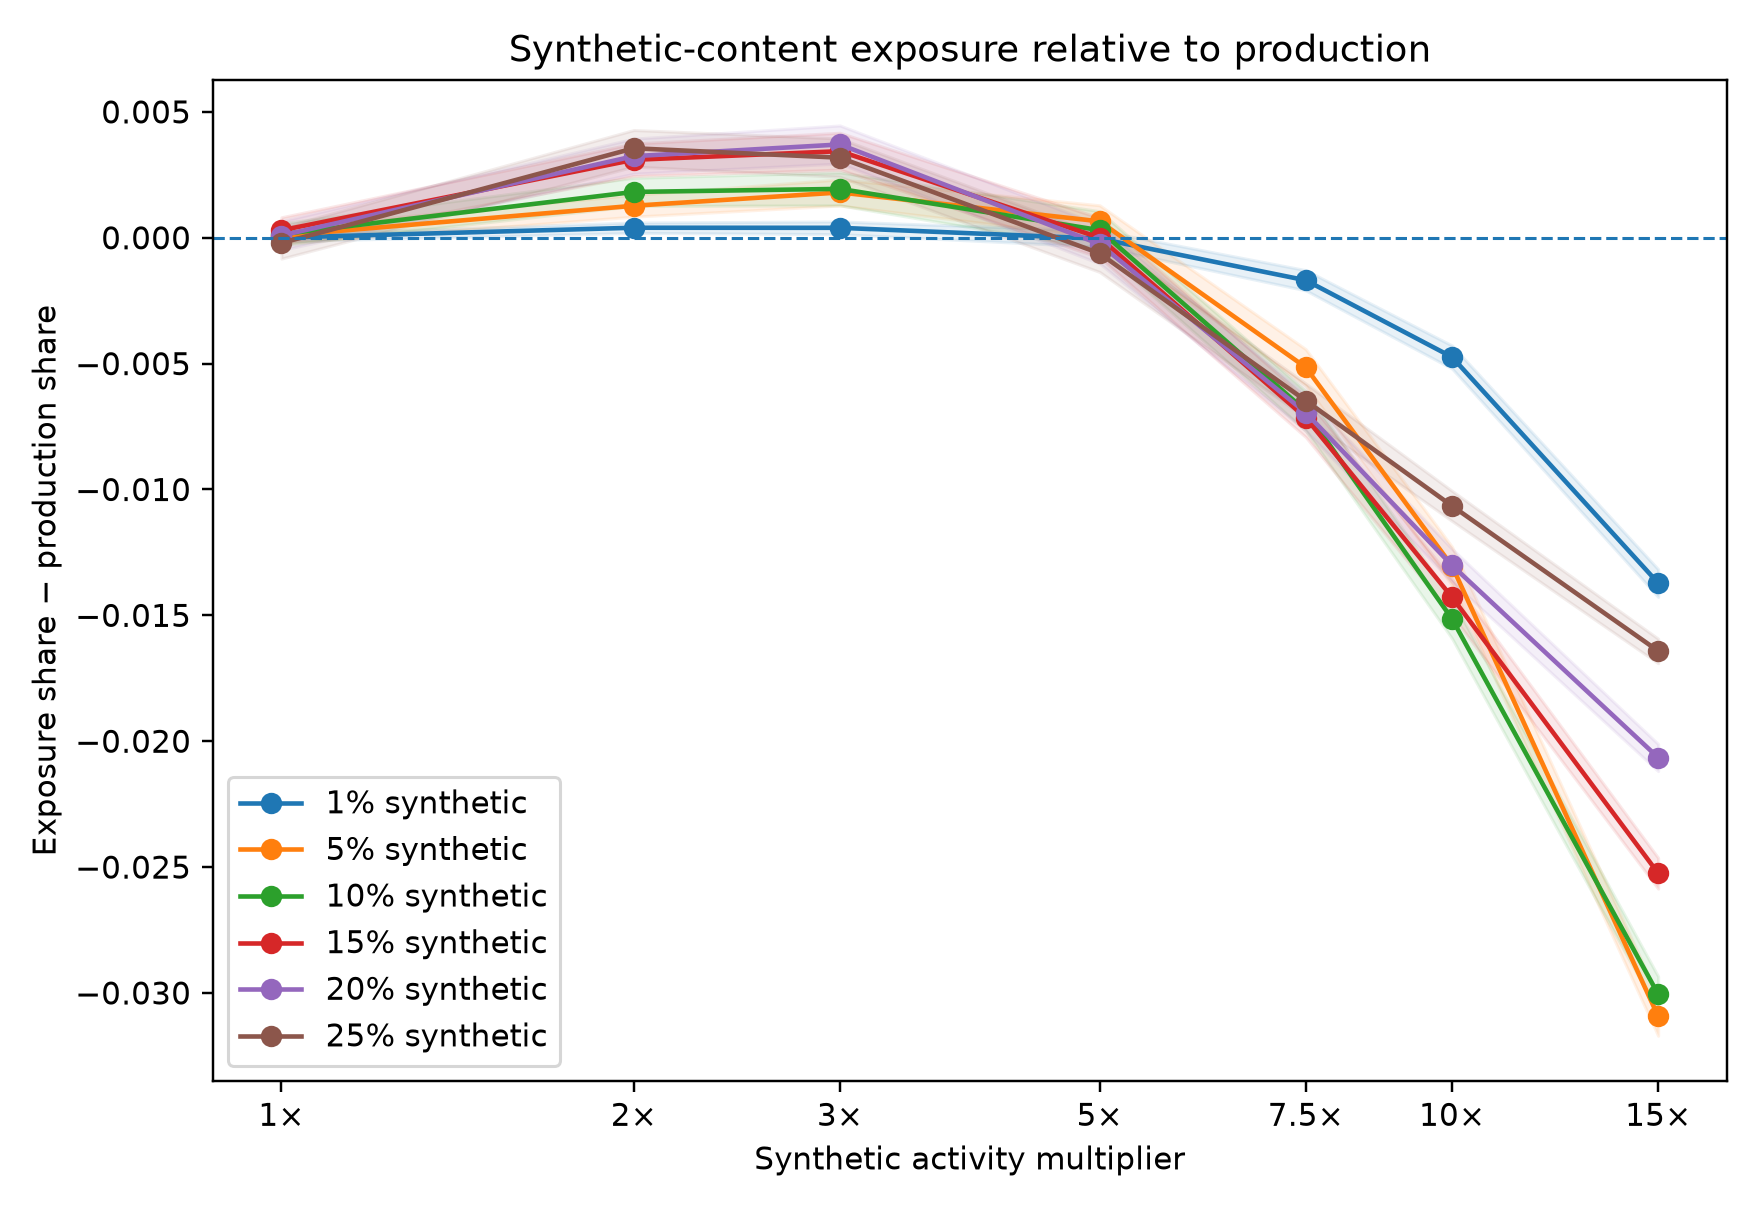
\includegraphics[width=0.9\linewidth]{imgs/alpha/D_vs_activity.png}
    \caption{\textbf{Relative synthetic exposure as activity increases.} Mean \(D=S_{\mathrm{exposure}}-S_{\mathrm{production}}\) across 10,000 independent worlds for each synthetic-producer prevalence and activity multiplier. Positive values indicate disproportionate synthetic exposure and negative values indicate attenuation. Shaded regions show 95\% confidence intervals.}
    \label{fig:D_vs_activity}
\end{figure}

The same pattern is visible across the full parameter grid in Fig.~\ref{fig:D_heatmap}. The largest mean \(D\) occurs at either \(2\times\) or \(3\times\) activity depending on prevalence. At \(7.5\times\) activity and above, mean \(D\) is negative for all tested prevalence levels. The magnitude of the effect varies with prevalence, but the overall turnover from small positive relative exposure at moderate activity to attenuation at high activity is present throughout the tested range.

\begin{figure}
    \centering
    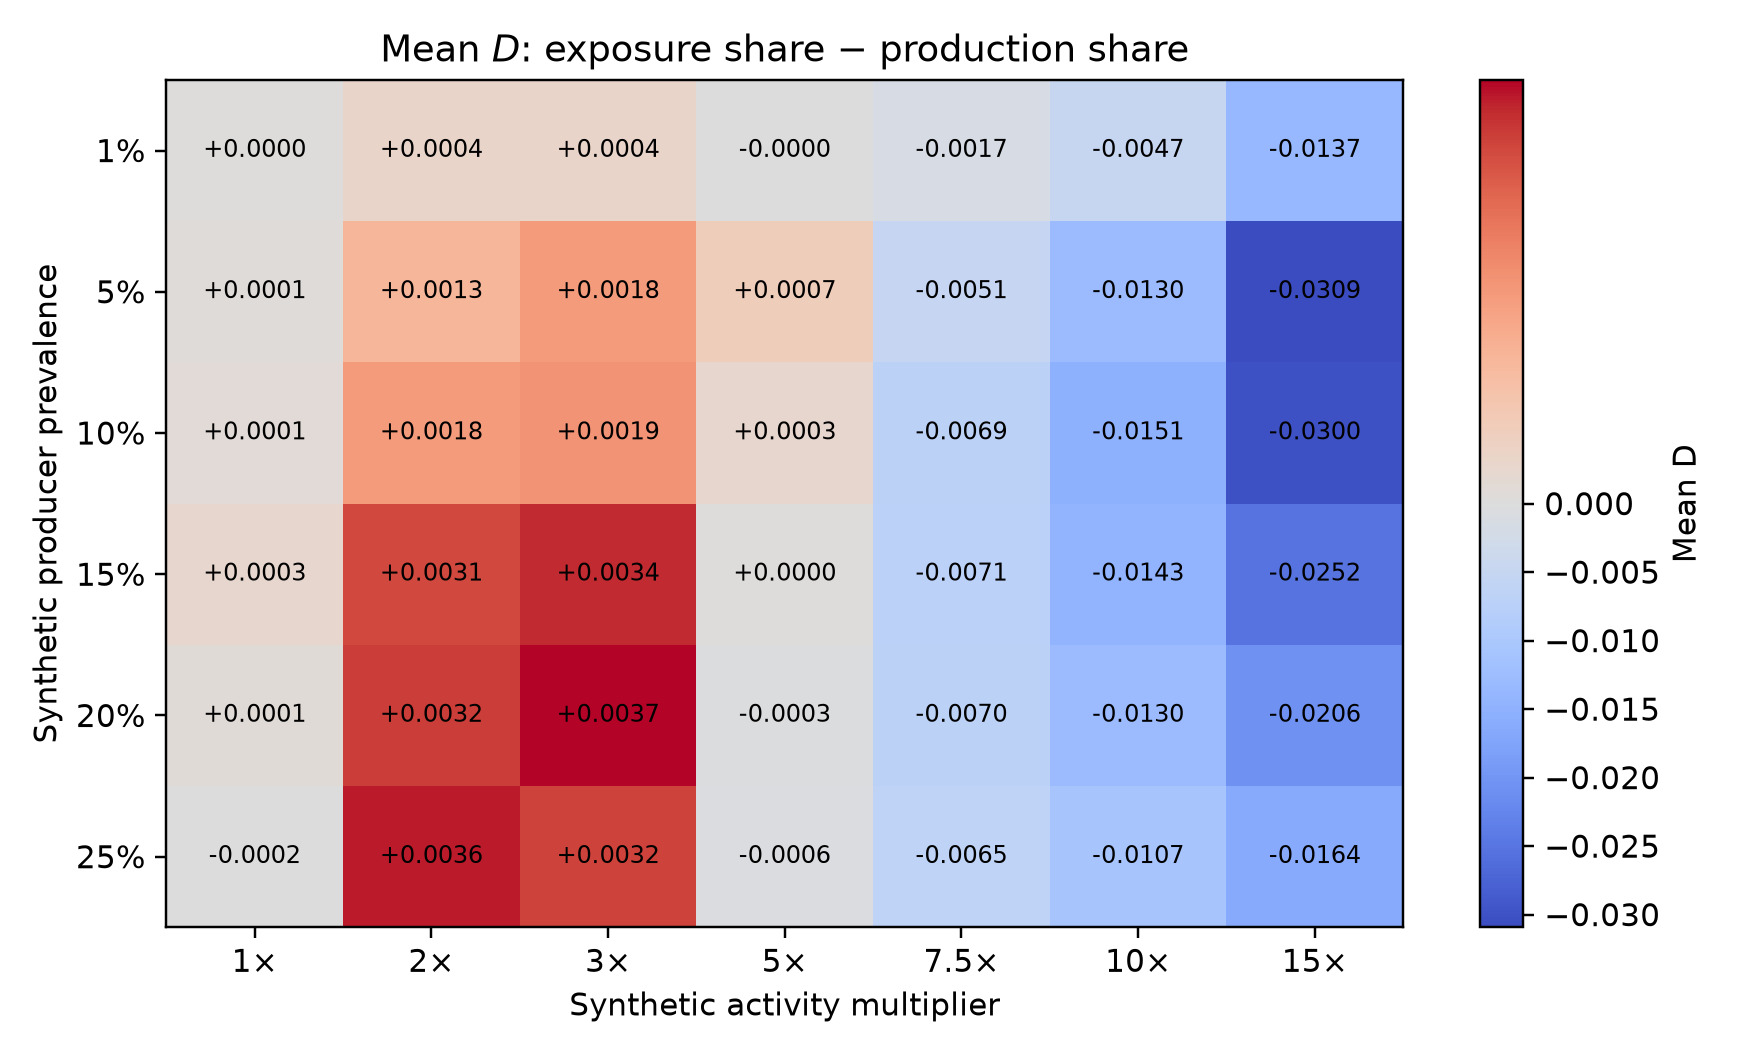
\includegraphics[width=0.9\linewidth]{imgs/alpha/D_heatmap.png}
    \caption{\textbf{Mean relative synthetic exposure across the experimental grid.} Each cell shows mean \(D=S_{\mathrm{exposure}}-S_{\mathrm{production}}\) across 10,000 independent worlds for the corresponding synthetic-producer prevalence and activity multiplier. Positive values indicate disproportionate exposure, while negative values indicate attenuation.}
    \label{fig:D_heatmap}
\end{figure}

The repeated-measures omnibus tests confirm that the relative-exposure outcome varies with both experimental factors. There is an effect of synthetic-producer prevalence, \(\chi^2(5)=869.53\), an effect of activity, \(\chi^2(6)=29176.50\), and a prevalence--activity interaction, \(\chi^2(30)=4042.40\); all three tests have \(p<0.001\). The interaction indicates that prevalence modifies the magnitude of the activity effect, although the qualitative non-monotonic pattern remains similar across prevalence levels.

The location of the turnover is also consistent across prevalence levels. The tested activity level with the largest mean \(D\) is \(2\times\) or \(3\times\), and linear interpolation between adjacent tested conditions places the subsequent zero crossing between \(4.67\times\) and \(5.28\times\). These values are descriptive interpolations within the simulated parameter grid rather than estimates of a universal threshold.

\begin{table}[t]
    \centering
    \caption{Turnover in mean relative exposure by synthetic-producer prevalence. Zero crossings are linearly interpolated between adjacent tested activity levels.}
    \label{tab:turnover}
    \begin{tabular}{rccc}
    \hline
    Prevalence & Peak activity & Peak mean \(D\) & Zero crossing \\
    \hline
    1\%  & \(2\times\) & 0.0004 & \(4.84\times\) \\
    5\%  & \(3\times\) & 0.0018 & \(5.28\times\) \\
    10\% & \(3\times\) & 0.0019 & \(5.11\times\) \\
    15\% & \(3\times\) & 0.0034 & \(5.00\times\) \\
    20\% & \(3\times\) & 0.0037 & \(4.87\times\) \\
    25\% & \(2\times\) & 0.0036 & \(4.67\times\) \\
    \hline
    \end{tabular}
\end{table}

The paired within-world contrasts support the same decline beyond the moderate activity peak. Table~\ref{tab:paired_3x_15x} reports the change in \(D\) from \(3\times\) to \(15\times\) activity. Mean \(D\) decreases at every tested prevalence, with the largest decline occurring at 5\% and 10\% prevalence. All reported contrasts remain significant after Holm adjustment, while the effect sizes indicate that the high-activity decline is substantially larger than the small positive exposure excess observed around the peak.

\begin{table}[t]
    \centering
    \caption{Paired within-world change in relative exposure from
    \(3\times\) to \(15\times\) synthetic activity. Negative values indicate
    lower \(D\) at \(15\times\). All contrasts have Holm-adjusted
    \(p<0.001\).}
    \label{tab:paired_3x_15x}
    \begin{tabular}{rccc}
    \hline
    Prevalence & Mean \(\Delta D\) & 95\% CI & \(d_z\) \\
    \hline
    1\%  & -0.0141 & [-0.0147,\,-0.0135] & -0.481 \\
    5\%  & -0.0327 & [-0.0336,\,-0.0318] & -0.721 \\
    10\% & -0.0320 & [-0.0329,\,-0.0311] & -0.685 \\
    15\% & -0.0287 & [-0.0296,\,-0.0278] & -0.614 \\
    20\% & -0.0244 & [-0.0252,\,-0.0235] & -0.539 \\
    25\% & -0.0196 & [-0.0205,\,-0.0187] & -0.444 \\
    \hline
    \end{tabular}
\end{table}

The original post-level diagnostics show lower synthetic receipts per accepted post at high activity and a larger fraction of synthetic posts with no receipts. The efficiency-gap sign agrees with \(D\) by construction, so it is not independent causal evidence. Checkpoint analysis also shows that, by 5,000 worlds, the maximum deviation of condition means from the final 10,000-world means is below 0.001. Full diagnostic figures and convergence outputs remain available with the activity-only report and research data. We retain the primary activity curves and contrasts here to focus on the new policy comparison.

\FloatBarrier
\subsection{Adaptive producers: matched policy comparisons}
\label{sec:adaptive-results}

The follow-up completes all 7,200 planned runs, with 200 worlds in each of 36 conditions. For SQ2, Fig.~\ref{fig:adaptive-main} compares content policies at matched activity and prevalence. Mean \(D\) for adaptive producers is negative throughout the one-item-feed grid. All 16 mean adaptive-minus-control changes in this grid are also negative. Six comparisons have Holm-adjusted \(p<0.05\) after correction across the complete family of 24 policy contrasts (Table~\ref{tab:adaptive-main}). This does not support an exposure-share advantage relative to production for the tested adaptive rule.

\begin{figure}[!htbp]
\centering
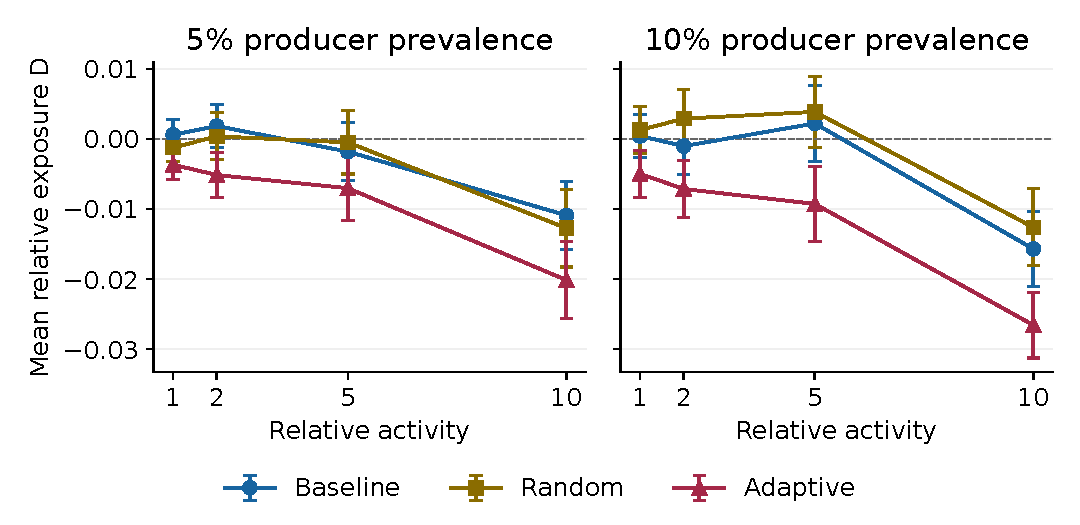
\includegraphics[width=\linewidth]{imgs/adaptive/policy_comparison.pdf}
\caption{\textbf{Content policies with a one-item feed.} Means and pointwise 95\% intervals across 200 paired worlds. Activity, producer identities and initial world state are matched between policies. Lines connect tested activities; they do not estimate a turnover threshold.}
\label{fig:adaptive-main}
\end{figure}
\begin{table}[!htbp]
\caption{Paired effect of content adaptation with a one-item feed (200 worlds). Changes are adaptive minus the stated control. Intervals are pointwise 95\% $t$ intervals; $p$ values use Holm adjustment across all 24 policy contrasts, including larger feeds.}
\label{tab:adaptive-main}
\centering\small\setlength{\tabcolsep}{4pt}
\begin{tabular}{rrlrrl}
\hline
Prevalence & Activity & Control & Mean $\Delta D$ & 95\% CI & Adjusted $p$ \\
\hline
5\% & 1$\times$ & baseline & -0.0043 & [-0.0074, -0.0011] & 0.128 \\
5\% & 1$\times$ & random & -0.0024 & [-0.0052, 0.0003] & 0.648 \\
5\% & 2$\times$ & baseline & -0.0070 & [-0.0113, -0.0027] & 0.030 \\
5\% & 2$\times$ & random & -0.0055 & [-0.0102, -0.0009] & 0.298 \\
5\% & 5$\times$ & baseline & -0.0052 & [-0.0109, 0.0005] & 0.643 \\
5\% & 5$\times$ & random & -0.0065 & [-0.0128, -0.0003] & 0.498 \\
5\% & 10$\times$ & baseline & -0.0092 & [-0.0157, -0.0027] & 0.100 \\
5\% & 10$\times$ & random & -0.0074 & [-0.0144, -0.0004] & 0.498 \\
10\% & 1$\times$ & baseline & -0.0054 & [-0.0100, -0.0008] & 0.321 \\
10\% & 1$\times$ & random & -0.0063 & [-0.0108, -0.0017] & 0.128 \\
10\% & 2$\times$ & baseline & -0.0061 & [-0.0120, -0.0003] & 0.498 \\
10\% & 2$\times$ & random & -0.0100 & [-0.0159, -0.0042] & 0.020 \\
10\% & 5$\times$ & baseline & -0.0115 & [-0.0184, -0.0046] & 0.026 \\
10\% & 5$\times$ & random & -0.0131 & [-0.0203, -0.0060] & 0.008 \\
10\% & 10$\times$ & baseline & -0.0109 & [-0.0175, -0.0042] & 0.029 \\
10\% & 10$\times$ & random & -0.0140 & [-0.0201, -0.0078] & $<0.001$ \\
\hline
\end{tabular}
\end{table}


At 10\% prevalence and \(10\times\) activity, the adaptive-minus-baseline change in \(D\) is \(-0.0109\), with pointwise 95\% interval \([-0.0175,-0.0042]\) and Holm-adjusted \(p=0.029\). Against the random-bin control, the change is \(-0.0140\), with interval \([-0.0201,-0.0078]\) and adjusted \(p<0.001\). At 5\% prevalence, the \(10\times\) comparison with baseline has a negative mean change of \(-0.0092\), but adjusted \(p=0.100\). We therefore do not generalize the resolved policy effects to every condition.

Lower relative exposure coexists with a larger synthetic receipt share. At 10\% prevalence and \(10\times\) activity, mean production share rises from 0.5257 under baseline to 0.5619 under adaptation. Mean receipt share rises from 0.5100 to 0.5353. The production-share increase is larger, yielding the negative paired change in \(D\). The adaptive subgroup therefore receives a larger share of receipts in this example even though its exposure falls further below its production share.

\subsubsection{Acceptance, efficiency and strategy choices}

Table~\ref{tab:adaptive-diagnostics} separates the relevant outcomes. At 10\% prevalence and \(10\times\) activity, mean posting acceptance rises from 0.5001 to 0.5786. The paired increase is 0.0785, with descriptive pointwise interval \([0.0750,0.0820]\). Receipts per attempted innovation increase by 0.5230, with interval \([0.3616,0.6844]\). Receipts per accepted post instead decrease by 0.3160, with interval \([-0.6192,-0.0128]\). The corresponding zero-receipt-frequency difference is \(-0.0023\), with interval \([-0.0106,0.0060]\), which does not resolve a change. These diagnostics are descriptive; their intervals are not multiplicity-adjusted.

\begin{table}[!htbp]
\caption{Mechanism diagnostics: adaptive minus baseline, with a one-item feed. $A_s$ is posting acceptance, $E_s$ is receipts per accepted post, $U_s$ is receipts per attempt, and $C$ is the late-minus-early change in mean per-producer maximum strategy share. These are descriptive paired mean differences.}
\label{tab:adaptive-diagnostics}
\centering\small
\begin{tabular}{rrrrrr}
\hline
Prevalence & Activity & $\Delta A_s$ & $\Delta E_s$ & $\Delta U_s$ & $\Delta C$ \\
\hline
5\% & 2$\times$ & 0.0811 & -0.4154 & 0.4744 & 0.1089 \\
5\% & 10$\times$ & 0.0788 & -0.0708 & 0.6329 & 0.0278 \\
10\% & 2$\times$ & 0.0791 & -0.7632 & 0.2646 & 0.1120 \\
10\% & 10$\times$ & 0.0785 & -0.3160 & 0.5230 & 0.0423 \\
\hline
\end{tabular}
\end{table}


Figure~\ref{fig:strategy-choices} shows early and late strategy frequencies. Pooled bin shares remain close to uniform because different producers can favour different bins. Individual choices are nevertheless much more concentrated under the adaptive rule. For the same 10\%--\(10\times\) condition, the mean per-producer maximum bin share increases from 0.8396 in the first quarter to 0.8816 in the last quarter, compared with 0.3562 to 0.3559 under baseline. The adaptive-minus-baseline difference in this change is 0.0423. The policy already concentrates choices early in the run; concentration alone is not evidence of better diffusion or successful optimization.

\begin{figure}[!htbp]
\centering
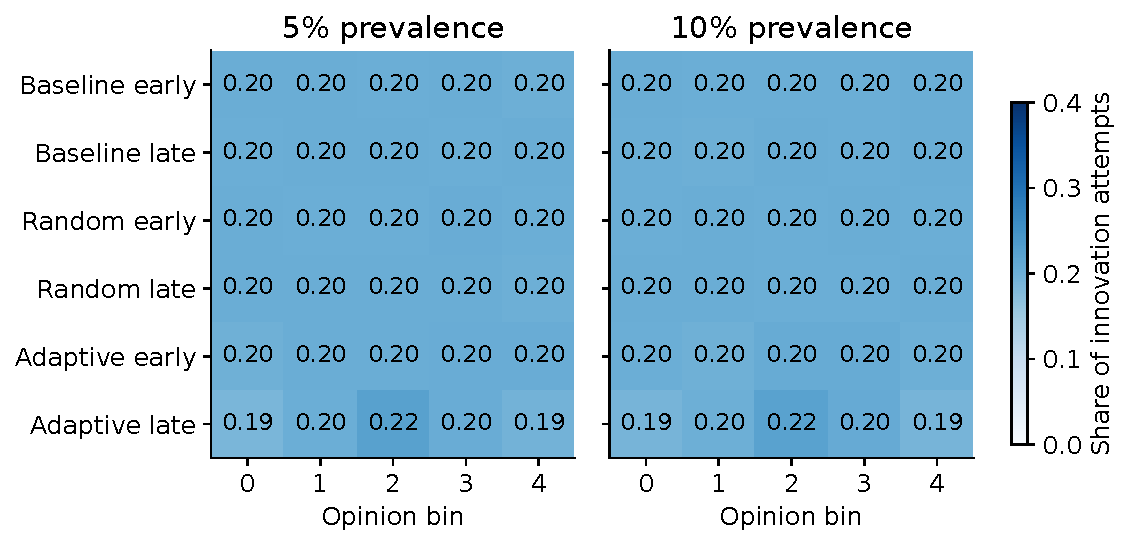
\includegraphics[width=\linewidth]{imgs/adaptive/strategy_choices.pdf}
\caption{\textbf{Strategy selections over time at \(10\times\) activity.} Each row shows the share of synthetic innovation attempts in five opinion bins, pooled across 200 worlds within the first or last quarter. Bin 0 spans \([-1,-0.6)\), and bin 4 spans \([0.6,1]\). Near-uniform pooled shares can conceal concentrated choices by different individual producers.}
\label{fig:strategy-choices}
\end{figure}

\subsubsection{Policy--activity interaction}

For SQ3, we compare the policy effect at \(10\times\) with its effect at \(2\times\), using paired differences within each world. No interaction contrast excludes zero at the pointwise 95\% level, and all eight Holm-adjusted \(p\) values equal 1.000. For adaptive versus baseline with a one-item feed, the mean interaction is \(-0.0022\) at 5\% prevalence and \(-0.0048\) at 10\% prevalence (Table~\ref{tab:adaptive-interaction}). The experiment does not resolve whether the adaptation effect changes between moderate and high activity. It also does not establish equivalence or rule out a smaller interaction.

\begin{table}[!htbp]
\caption{Does the adaptation effect change from 2$\times$ to 10$\times$ activity? Each estimate is $(D_{\rm adaptive}-D_{\rm baseline})_{10}-(D_{\rm adaptive}-D_{\rm baseline})_2$, paired within world. Intervals are pointwise; Holm correction covers all eight interaction contrasts, including the random control.}
\label{tab:adaptive-interaction}
\centering\small
\begin{tabular}{rrrrl}
\hline
Prevalence & Feed & Mean interaction & 95\% CI & Adjusted $p$ \\
\hline
5\% & 1 & -0.0022 & [-0.0101, 0.0056] & 1.000 \\
10\% & 1 & -0.0048 & [-0.0138, 0.0042] & 1.000 \\
5\% & 3 & -0.0039 & [-0.0114, 0.0035] & 1.000 \\
5\% & 5 & 0.0034 & [-0.0039, 0.0107] & 1.000 \\
\hline
\end{tabular}
\end{table}


\FloatBarrier
\subsection{Feed-capacity sensitivity}
\label{sec:feed-results}
\subsubsection{Activity-only capacity experiment}

The separate activity-only capacity experiment contains all 3,600 planned runs, with 200 worlds distinct from the adaptive experiment. Figure~\ref{fig:feed-capacity} and Table~\ref{tab:feed-capacity} show substantial capacity dependence. At \(15\times\), mean \(D\) is negative in all six prevalence--capacity combinations. For example, at 5\% prevalence it is \(-0.0304\) with a one-item feed, \(-0.0050\) with a five-item feed, and \(-0.0508\) with a 20-item feed. Increasing capacity therefore does not simply weaken attenuation.

\begin{figure}[!htbp]
\centering
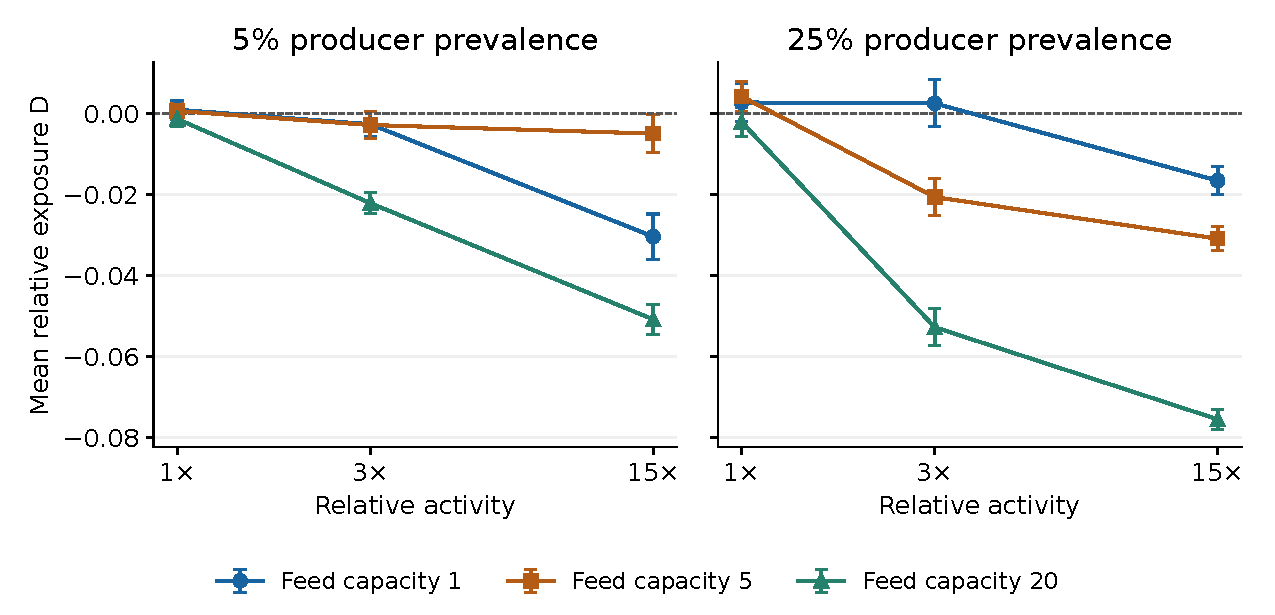
\includegraphics[width=\linewidth]{imgs/robustness/feed_capacity.pdf}
\caption{\textbf{Feed-capacity sensitivity.} Mean relative exposure and pointwise 95\% confidence intervals across 200 independent paired worlds. Lines connect the three tested activity levels for readability; they do not estimate intermediate values or a turnover threshold.}
\label{fig:feed-capacity}
\end{figure}

\begin{table}[!htbp]
\caption{Feed-capacity sensitivity across 200 paired worlds. Condition means and paired changes in $D$ use the same worlds. Intervals are pointwise 95\% $t$ intervals, without multiplicity adjustment.}
\label{tab:feed-capacity}
\centering\small
\begin{tabular}{rrrrrl}
\hline
Prevalence & $\alpha$ & Mean $D_3$ & Mean $D_{15}$ & Mean change & 95\% CI \\
\hline
5\% & 1 & -0.0027 & -0.0304 & -0.0277 & [-0.0336, -0.0218] \\
5\% & 5 & -0.0028 & -0.0050 & -0.0021 & [-0.0077, 0.0034] \\
5\% & 20 & -0.0221 & -0.0508 & -0.0287 & [-0.0330, -0.0244] \\
25\% & 1 & 0.0025 & -0.0166 & -0.0191 & [-0.0256, -0.0126] \\
25\% & 5 & -0.0206 & -0.0309 & -0.0103 & [-0.0154, -0.0052] \\
25\% & 20 & -0.0527 & -0.0755 & -0.0227 & [-0.0275, -0.0179] \\
\hline
\end{tabular}
\end{table}


All six mean paired contrasts \(D_{15}-D_3\) are negative. Five pointwise intervals exclude zero. For the five-item feed at 5\% prevalence, however, the mean change is \(-0.0021\), with interval \([-0.0077,0.0034]\); this comparison does not resolve a decline. At 25\% prevalence the same contrast is \(-0.0103\), with interval \([-0.0154,-0.0052]\). These exploratory intervals have no multiplicity adjustment.

The small positive effect at moderate activity in the main sweep is not consistently reproduced in the sensitivity sample. With a 20-item feed, mean \(D_3\) is already negative at both prevalences. The 200-world one-item-feed sample also does not resolve the small positive \(D_3\) seen in the 10,000-world sweep. The focused experiment therefore supports high-activity attenuation in the tested settings, but not a capacity-independent moderate-activity peak or zero crossing near \(5\times\).

\subsubsection{Adaptive-policy capacity comparison}

The new capacity comparison uses the same 200 paired worlds as the adaptive main grid, at 5\% prevalence and activities \(2\times\) and \(10\times\). Figure~\ref{fig:adaptation-capacity} shows the adaptive-minus-control effects at capacities 1, 3 and 5. All eight policy contrasts at capacities 3 and 5 have pointwise intervals containing zero, and all adjusted \(p\) values exceed 0.60.

For example, at capacity 3 and \(10\times\) activity, the adaptive-minus-baseline mean change in \(D\) is \(-0.0060\), with interval \([-0.0123,0.0003]\). At capacity 5 it is 0.0009, with interval \([-0.0048,0.0067]\). We do not resolve a policy effect in these larger-feed conditions. This uncertainty does not establish that their policy effects differ from the one-item-feed effects; comparing significance across conditions is not a test of a capacity--policy interaction.

\begin{figure}[!htbp]
\centering
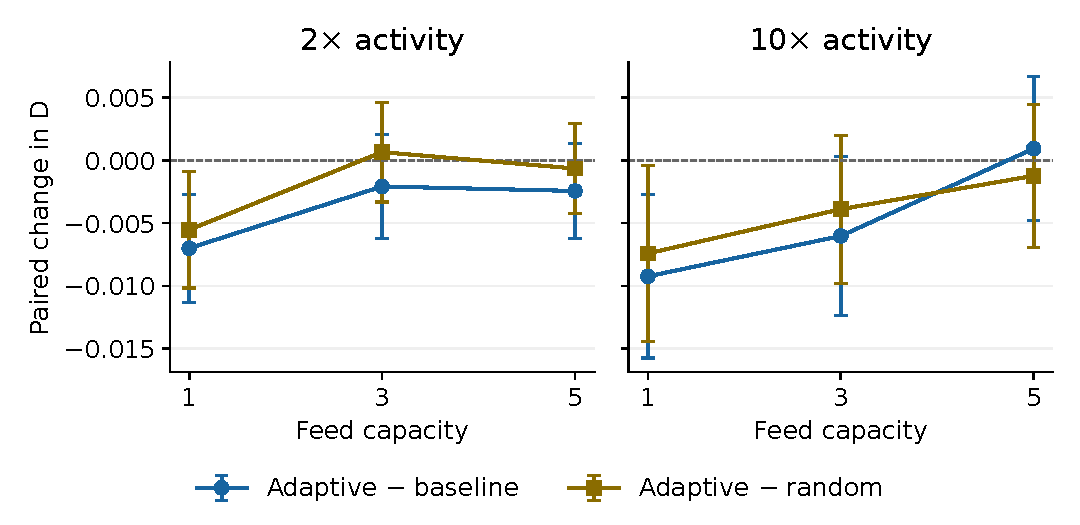
\includegraphics[width=\linewidth]{imgs/adaptive/adaptation_capacity.pdf}
\caption{\textbf{Adaptive-policy sensitivity to feed capacity at 5\% prevalence.} Paired changes in \(D\) and pointwise 95\% intervals across 200 worlds. Each point compares adaptation with the stated control at the same activity and capacity.}
\label{fig:adaptation-capacity}
\end{figure}

\FloatBarrier
\section{Discussion}

For SQ1, the original activity-only sweep distinguishes absolute prevalence of synthetic-origin content from exposure relative to production. High activity raises both production and receipt shares, even when mean \(D\) becomes negative. A negative value therefore does not imply that synthetic content has become rare or that total receipts have fallen. The interpolated crossing near \(5\times\) describes the original one-item-feed configuration, not a universal activity threshold.

For SQ2, the specified feedback rule changes exposure without producing an advantage in exposure share relative to production in the one-item-feed grid. The clearest high-activity example shows why the attempt measurements matter: posting acceptance and receipts per attempt increase, while receipts per accepted post decrease. The extra accepted output can raise the subgroup's receipt share even when \(D\) falls. We therefore cannot treat a negative \(D\) as evidence that the producer receives less attention in every sense, or treat higher receipt share as evidence of disproportionate amplification.

The adaptive rule is operationally different from high activity alone. It uses past receipt outcomes, and the implementation tests show that changing those outcomes changes future bin choices. The observed concentration of individual choices is consistent with strong exploitation of earlier successes. However, responsiveness to feedback does not guarantee improved performance. Delayed cascades, sparse exploration, changing network conditions and age differences among posts can make a cumulative per-post score favour choices that do not improve overall exposure efficiency.

For SQ3, we do not resolve an interaction between policy and activity over the tested \(2\times\)--\(10\times\) contrast. We also do not resolve the adaptive effect at capacities 3 and 5. These uncertain estimates limit transfer of the one-item-feed comparisons; they do not prove that capacity has removed an effect or that the policy is equivalent to its controls. The separate activity-only capacity experiment further shows that a simple limited-attention explanation is insufficient to identify the underlying mechanism.



The extension creates a direct connection to the feedback-responsive production described by Tang et al.~\cite{tang2026} and the creation--distribution--reward cycle discussed by Pendergrass et al.~\cite{pendergrass2025}. Producers now use past distribution outcomes to select future content opinions. This is a model of one feedback component, not a test of the full empirical accounts. Actual production includes formats, costs, account coordination and monetization that the scalar opinion model does not represent.

The receiving rule also constrains interpretation. Because it depends on sender and recipient opinions rather than directly on the new content opinion, a learned opinion choice is not equivalent to optimizing a real recommendation ranking. Its effect arises through posting acceptance, reposting, opinion change and network evolution. These coupled mechanisms can produce an outcome that differs from the producer's receipt-per-post objective. The model permits that outcome; it does not guarantee that an adaptive policy outperforms a non-adaptive one.

\subsection{Limitations and future work}

The five bins, exploration probability, cumulative reward estimate and event horizon are modelling choices, not empirical calibrations. Individual producers can make relatively few original-content attempts during 100,001 activations. Consequently, early reward differences and limited exploration can matter. Scores include all historical receipts with no forgetting and do not control for post age. Older content has more time to acquire feedback, while recent posts are right-censored. We also assume complete provenance-attributed receipt feedback. Testing delayed or partial observation, age-matched rewards, different exploration rates and a forgetting window would assess these policy assumptions.

The feedback objective is conditional on a post being accepted. Comparing an objective based on receipts per attempt would help determine whether a producer should account explicitly for rejected creation attempts. Our measurements separate acceptance, receipts per accepted post and receipts per attempt, but do not identify their contributions through an independent causal mediation analysis. We also do not interpret a non-significant contrast as evidence that adaptation has no effect.

The original 10,000-world sweep estimates the activity-only model precisely. The adaptive follow-up uses 200 worlds and a smaller parameter grid, so it has different Monte Carlo uncertainty and cannot estimate a new turnover threshold. The additional capacity comparison covers only 5\% prevalence and two activity levels. Neither precision nor robustness across these few settings validates the model against real platform data.

Other external-validity limits remain: a random follower network, a stylised opinion-based receiving filter, common innovation probabilities and uncalibrated opinion dynamics. Capacity changes retention, repost order, duplicate suppression and initial background stock together. We therefore do not identify attention scarcity or feed displacement as the cause of a result. Alternative networks, recommendation rules, longer horizons and initialization controls require separate experiments.

The model still does not represent generative media quality, visual formats, semantic topics, coordinated ownership, financial incentives or actual engagement. The synthetic label marks a producer subgroup and its provenance; a generic high-activity group using the same strategy could produce the same outcomes. These limitations separate the demonstrated computational feedback rule from claims about real AI-slop producers.

\section{Conclusion}

The original 10,000-world sweep answers SQ1: higher producer activity raises synthetic production and receipt shares, but relative exposure falls at high activity in the one-item-feed configuration.

The 200-world, 7,200-run follow-up answers SQ2 for a specified feedback rule. Adaptive producers select opinion bins using past receipts per accepted post. All mean adaptive-minus-control changes in \(D\) are negative with a one-item feed, although many remain uncertain after correction. At 10\% prevalence and \(10\times\) activity, adaptation raises production share by 0.0363 and receipt share by 0.0254, lowering \(D\) by 0.0109. Higher posting acceptance and receipts per attempt therefore coexist with lower exposure per accepted post.

For SQ3, the policy--activity interaction and larger-feed policy effects remain unresolved. These estimates neither establish equivalence nor rule out smaller effects. Our contribution is a tested distinction between more accepted output, more receipts per attempt and disproportionate exposure. The results concern one cumulative-feedback policy over a finite horizon, not actual media quality, engagement, coordinated accounts or real platform ranking.

\bibliographystyle{splncs04}
\bibliography{bibliography-adaptive}
%
\end{document}
